% !TeX root = ../Book4.tex
\begin{figure}[htbp]
	\centering
	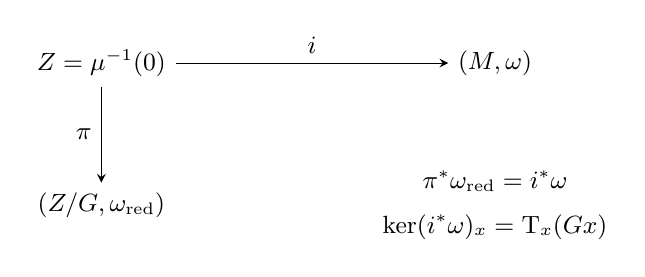
\begin{tikzpicture}[font=\small,>=stealth]
		\node (Z) at (0,1.5) {\(Z=\mu^{-1}(0)\)};
		\node (M) at (5,1.5) {\((M,\omega)\)};
		\node (B) at (0,-0.3) {\((Z/G,\omega_{\mathrm{red}})\)};
		\draw[->] (Z)--node[above] {\(i\)} (M);
		\draw[->] (Z)--node[left] {\(\pi\)} (B);
		\node[align=center] at (5,-0.3) {\(\pi^*\omega_{\mathrm{red}}=i^*\omega\)\\[5pt]\(\ker(i^*\omega)_x=\mathrm{T}_x(Gx)\)};
	\end{tikzpicture}
	\caption[水平集与轨道商]{先把辛形式限制到矩映射的零水平，再沿群轨道取商。限制型的核恰为商映射消去的方向，所以商上的形式非退化。}
	\label{g4:fig:1002:reduction-diagram}
\end{figure}
